\chapter{Proiectare rețele profile}\label{chapter:proiectare}

\section{Rețele de profile subțiri}

\subsection{Calculul diametrului la butuc}

Pentru a calcula diametrul la butuc conform teoriei dezvoltata la Timișoara de Susan-Resiga et al \cite{susanhub} trebuie sa rezolvam ecuația pentru intensitatea rotației $\sigma$, cu un rezultat adimensional.

Conform ecuației fundamentale a turbomașinilor (ecuația lui Euler) avem viteza absolută la periferie:

\begin{equation}
gH=UV_{u}, \text{ sau } gH=\frac{\pi n}{30} R_{p} V_{up} \Rightarrow V_{u}=\frac{30gH}{\pi n R_{p}}
\end{equation}

Viteza medie de descărcare este:

\begin{equation}
V_{ad}=\frac{Q}{\pi R_{p}^2}
\end{equation}

În ambele ecuații, (2.1) și (2.2) raza conductei este practic raza de la periferie a turbinei. Ca rezultat, parametrul de intensitate a rotației este:

\begin{equation}
\sigma \equiv \frac{V_{up}}{V_{ad}} = 30 \frac{g H R_{b}}{n Q}
\end{equation}

În care regiunea (necunoscută) stagnantă $R_{s}$ (la butuc), se indică raportul de raza de stagnare fata de raza la periferie, totul la pătrat, de unde putem obține $x$ și apoi raza la butuc:

\begin{equation}
x \equiv \bigg(\frac{R_{s}}{R_{p}}\bigg)^2 \Rightarrow R_{s} = \sqrt{x} R_{p}
\end{equation}

Pentru o turbionare cu circulație constantă și o presiune totală constantă în conducta a fost derivata \cite{susanhub} o ecuație algebrică care se aplica pentru $\sigma$ și $x$:

\begin{equation}
\frac{\sigma^2}{x^2} - \frac{2}{(1-x^3)} = 0
\end{equation}

Din (2.4) și (2.5) putem calcula raza la butuc $R_{s}$ folosind \cite{lebedev1991formulae} și obținem o valoare de $94\si{mm}$.

\clearpage


\subsection{Calcule teoretice a vitezelor}

Considerăm zona de interacțiune a turbinei cu fluidul în trei porțiuni:
\begin{itemize}
	\item prima zonă numită zonă amonte stator ZAS
	\item a doua porțiune: zona stator-rotor numită de acum ZSR
	\item zona trei sau zona aval rotor ZAR
\end{itemize}

La ZAS avem viteza axială $V_{a}$ care se menține pe toate cele trei porțiuni considerate ale turbinei, iar valoarea acesteia este:

\begin{equation}
V_a=\frac{Q}{\pi(R_{p}^2-R_{b}^2)}=6.8\si{m/s}
\end{equation}\\

\În ZSR, avem viteza tangențiala $U$:

\begin{equation}
U=\omega R \text{ sau } \frac{\pi n}{30} \frac{R_{b} + R_{p}}{2}=16.0\si{m/s}
\end{equation}

Conform ecuației fundamentale a turbomașinilor (ecuația lui Euler) avem viteza absolută:

\begin{equation}
gH=UV_{u}, \text{ sau } gH=\frac{\pi n}{30} \frac{R_{b}+R_{p}}{2} V_{u} \Rightarrow V_{u} = \frac{30gH}{\pi n} \frac{2}{R_{b}+R_{p}} = 14.7\si{m/s}
\end{equation}


Unghiul $\alpha_2$ dintre direcția tangențială și viteza absolută $V_u$ este:

\begin{equation}
arctan(\alpha_{2 })=\frac{V_{a}}{V_{u}} \Rightarrow \alpha_{2}=24.9\si{\degree}
\end{equation}



Unghiul $\beta_2$ dintre direcția tangențială și viteza relativă $W_2$ este:

\begin{equation}
arctan(\beta_{2})=\frac{V_{a}}{U - V_{u}} \Rightarrow \beta_{2} =79.0\si{\degree}
\end{equation}


\subsection{Triunghiurile de viteză}

Triunghiurile de viteză pentru ZSR arată în felul următor:

\begin{figure}[h!]
	\centering
	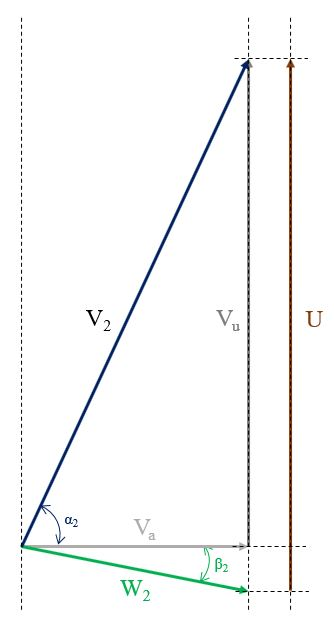
\includegraphics[scale=0.5]{figures/triunghi_viteza_ZSR.jpg}
	\caption{Triunghi viteză în zona stator-rotor}
	\label{Triunghi viteză în zona stator-rotor}
\end{figure}



Pentru ZAR avem aceleași viteză axială $V_a$ respectiv tangențială $U$. Putem calcula unghiul $\beta_3$ pentru a completa triunghiurile de viteză.

\begin{equation}
arctan(\beta_{3})=\frac{V_{a}}{U} \Rightarrow \beta_{3} =23.1\si{\degree}
\end{equation}

\begin{figure}[h!]
	\centering
	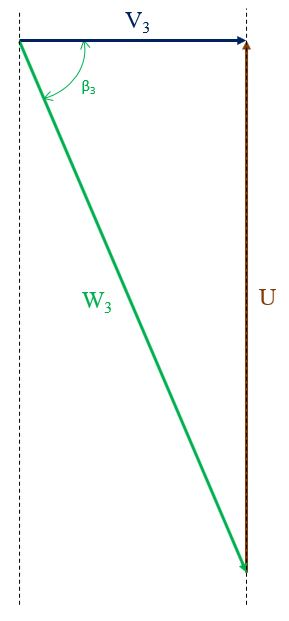
\includegraphics[scale=0.5]{figures/triunghi_viteza_ZAR.jpg}
	\caption{Triunghi viteză în zona aval rotor}
	\label{Triunghi viteză în zona aval rotor}
\end{figure}

\clearpage


\section{Adăugare funcție de grosime}

\subsection{Subsection}